\newpage
\subsection{Implementing FastCards}
\texHeader
\hypertarget{fastCard tex}{}

\begin{itemize}
  
\item[$\blacktriangleright$] Create a new eclass under ``LearningBoxLanguage" named
\texttt{FastCard} which extends \texttt{Card}. It doesn't need any new attributes, so leave its declaration empty. It should resemble Fig.~\ref{fig:fastClass}.

\vspace{0.5cm}

\begin{figure}[htp]
\begin{center}
  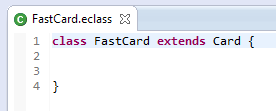
\includegraphics[width=0.45\textwidth]{eclipse_fastCardClass}
  \caption{\texttt{FastCard}s are a special type of \texttt{Card}}
  \label{fig:fastClass}
\end{center}
\end{figure}

\item[$\blacktriangleright$] Open \texttt{Partition.eclass} once again, and find \texttt{check(card, guess)}. Edit the activity by adding a second
\texttt{if/else} construct. Call the new assertion pattern \texttt{isFastCard}, and the action pattern \texttt{promoteFastCard}. Move the original
\texttt{[promoteCard]} pattern into the \texttt{else} statement. The check method should then resemble Fig.~\ref{fig:isFastCard}.

\vspace{0.5cm}

\begin{figure}[htp]
\begin{center}
  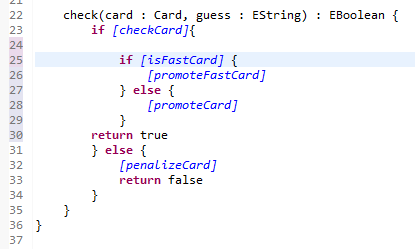
\includegraphics[width=0.7\textwidth]{eclipse_isFastCardFlow}
  \caption{Checking for \texttt{FastCard}s}
  \label{fig:isFastCard}
\end{center}
\end{figure}

\item[$\blacktriangleright$] \texttt{isFastCard} is a simple, one line statement pattern. You simply need to create a \emph{binding expression} to bind the
object variable \texttt{fastCard} of type \texttt{FastCard}, to \texttt{card} of type \texttt{Card} that was passed in as a parameter. Remember, to access
parameter values, prefix the name with a `\$' symbol. Your workspace should now resemble Fig.~\ref{fig:isFastCardPattern}.

\begin{figure}[htp]
\begin{center}
  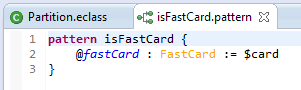
\includegraphics[width=0.5\textwidth]{eclipse_isFastCardPattern}
  \caption{A \texttt{FastCard} attribute constraint}
  \label{fig:isFastCardPattern}
\end{center}
\end{figure}

\item[$\blacktriangleright$] To establish \texttt{promoteFastCard}, first create the four main object variables: \texttt{@this} for the
current partition of the card, \texttt{@fastCard} representing the card, \texttt{lastPartition} for the last partition in the box, and the \texttt{box}
containing all partitions. Under \texttt{lastPartition}, also create a NAC \texttt{next}, to forbid that the last partition in the box has a next partition.
Your pattern should now resemble Fig.~\ref{fig:objVarFastCard}.

\vspace{0.5cm}

\begin{figure}[htp]
\begin{center}
  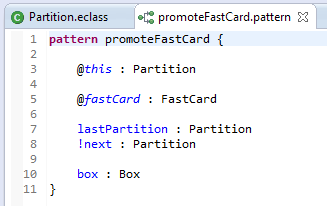
\includegraphics[width=0.6\textwidth]{eclipse_promoteFastCardObjVars}
  \caption{Object variables for \texttt{promoteFastCard}}
  \label{fig:objVarFastCard}
\end{center}
\end{figure}

\item[$\blacktriangleright$] When creating the necessary link variables remember - this is the pattern that will be invoked when the fast card status has
already been confirmed! This means that you'll want to:
(1) ensure that all partitions belong to the current box.
(2) remove \texttt{fastCard} from its current partition, and insert it into \texttt{lastPartition}
(3) confirm that \texttt{lastPartition} does not have a \texttt{next} partition, i.e., it really is the last partition in the box.\footnote{If you need help
remembering how NACs work, review Section 7}

\vspace{0.5cm}

\item[$\blacktriangleright$] Your final pattern should resemble Fig.~\ref{fig:promoFastCardFinal}. As you can see, this pattern is remarkably similar to the
original movement patterns, \texttt{pro\-mote\-Card} and \texttt{pen\-a\-lize\-Card} (Fig.~\ref{fig:completedPatterns}). This of course makes sense -- the
target pattern is only now always the last partition in the box and no longer the current \texttt{next}.

\newpage

\vspace*{1cm}

\begin{figure}[htp]
\begin{center}
  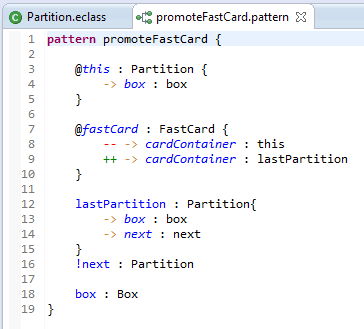
\includegraphics[width=0.6\textwidth]{eclipse_promoFastCardFinal}
  \caption{The completed fast card promotion pattern}
  \label{fig:promoFastCardFinal}
\end{center}
\end{figure}

\vspace{0.5cm}

\item[$\blacktriangleright$] You have now completed \emph{every} method signature using SDMs - fantastic work! Build your project to
confirm there aren't any errors, and review Fig.~\ref{fig:promoteFastCardPattern} to see how \texttt{FastCard}s are implemented in the visual syntax.

\item[$\blacktriangleright$] You are encouraged to read the visual SDM sections on each method to understand the full scope of eMoflon's features (which start
on page~\hyperlink{Page.9}{9}). 
  
\end{itemize}
